\pdfoutput=1
\documentclass[pra,twocolumn,showpacs,amsmath,amssymb]{revtex4-1}

\usepackage{graphicx}%Include figure files
\usepackage{dcolumn}%Align table columns on decimal point
\usepackage{bm}% bold math
\usepackage{subcaption}


%\nofiles

\begin{document}

\newcommand{\trel}{$\tau_A / \tau_B$}

\title{Project 1: Modelling Radioactive Decay}


\author{John Russo}
\affiliation{Department of Physics and Astronomy, University
of Delaware, Newark, DE 19716-2570, USA}

\begin{abstract}
Radioactive decay and resonance are numerically modeled using an Euler method
approach and compared to the exact solutions.
Stability of the numerical solutions to the radioactive decay problem are analyzed
for different timestep lengths. Dependence of long-term behavior of the $B$
population on the ratio of the populations' e-folding times \trel~is explored.
The long-term behavior of the resonant system is examined, and steady-state
behavior is confirmed.
\end{abstract}

\pacs{23.90.+w}


\maketitle





\section{Introduction} \label{sec:intro}

Modelling radioactive decay involves only a simple numerical solution to a
differential equation. However, it is a useful demonstration of basic numerical
solving techniques, with a wide range of applications.
Radioactive decay is a stochastic process where a nucleus breaks down, releasing
energy, matter, or both, depending on the type of decay.
Radioactive decay is a process studied for applications from nuclear weapons to
carbon dating, where understanding decay rates of isotopes can yield information
about age of a sample.

[TODO]: Findings of paper here



\section{Method}

\subsection{Part I - Decay}


In Part I of this project, numerical solutions are plotted for the case of two
populations of nuclei, $A$ and $B$. $A$ nuclei decay into $B$ nuclei. $B$
nuclei also decay.

Decay of these populations is governed by the following first-order coupled
differential equations

\begin{align}
  \frac{d N_A}{dt} &= -\frac{N_A}{\tau_A} \\
  \frac{d N_B}{dt} &= \frac{N_A}{\tau_A} - \frac{N_B}{\tau_B}
\end{align}

where $N_A$ and $N_B$ are the $A$ and $B$ nucleus populations, and $\tau_A$ and
$\tau_B$ are the respective e-folding times of the nuclei.

These equations can be normalized to

\begin{align}
  \frac{d \bar N_A}{d \bar t} &= - \bar N_A \label{eq:decay_A_norm}\\
  \frac{d \bar N_B}{d \bar t} &= \bar N_A - \frac{\tau_A}{\tau_B} \label{eq:decay_B_norm}\bar N_B
\end{align}

where bars indicate the normalized variables.

Numerical solutions are obtained by using the Euler method with a fixed time
interval $dt$. $dt$ will be varied to explore the stability of different length
time steps. Exact solutions are obtained by analytically solving the differential
equations of the populations in Mathematica for the given initial conditions
and plotting the solutions.

All numerical simulations of this system are performed with
$N_A (t=0) = 200$ and $N_B (t=0) = 5$. $dt$ for the stable simulations is chosen
to be $0.1$, but varied between higher values to explore instabilities/

\subsection{Part II - Resonance}

In Part II a system is analyzed where $B$ nuclei decay back into $A$ nuclei.
Since each species of nucleus can now decay into the other, this is no longer
truly a radioactive decay problem. This is more analogous to a resonance or
tunnelling problem, where particles tunnel between two states with equal energy.
This system is described by

\begin{align}
  \frac{d N_A}{dt} &= \frac{N_B}{2 \tau} - \frac{N_A}{\tau} \\
  \frac{d N_B}{dt} &= \frac{N_A}{\tau} - \frac{N_B}{2 \tau}
\end{align}

which are normalized to

\begin{align}
  \frac{d \bar N_A}{d \bar t} &= -  \bar N_A + \frac{1}{2} \bar N_B \label{eq:res_A_norm} \\
  \frac{d \bar N_B}{d \bar t} &=  \bar N_A - \frac{1}{2} \bar N_B \label{eq:res_B_norm}.
\end{align}

This system is simulated with $dt=0.1$, $N_A(0)=150$, and $N_B(0)=0$.



\section{Results}

\subsection{Part I - Radioactive Decay}\label{sec:decay}

Numerical solutions to the population equations from radioactive decay
 are shown in Fig.~\ref{fig:numerical} and can be compared to
a plot of the analytical solution to the differential equations of the systems
in Fig.~\ref{fig:analytical} to confirm accuracy of the numerical solutions.

Varying the parameter \trel~demonstrates its effect on the
system's transient and steady state behavior.
As can be seen in Eq.~\ref{eq:decay_B_norm}, the ratio
 \trel~only affects the decay of the $B$ population. The $A$
 population's rate of decay is determined solely by the size of the $A$ population.


 \begin{figure}
   \begin{subfigure}{.7\linewidth}
     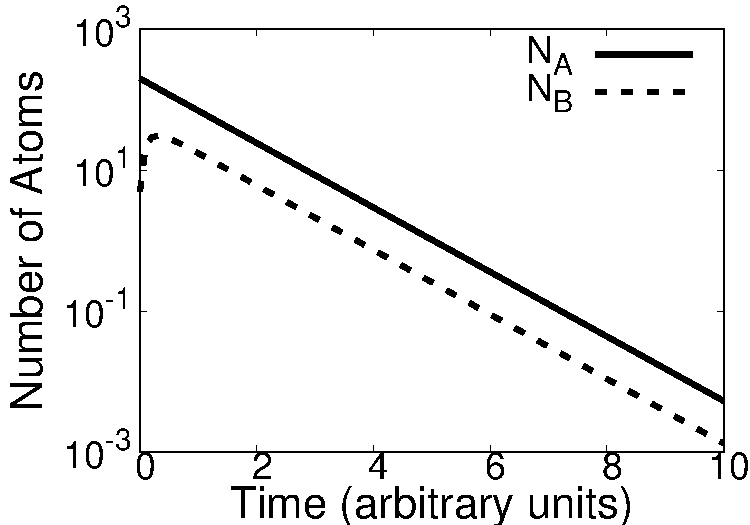
\includegraphics[width=\linewidth]{t_gt_1.pdf}
     \caption{$\tau_A / \tau_B=5$}
     \label{fig:tau_gt_1}
   \end{subfigure}
 ~
   \begin{subfigure}{.7\linewidth}
     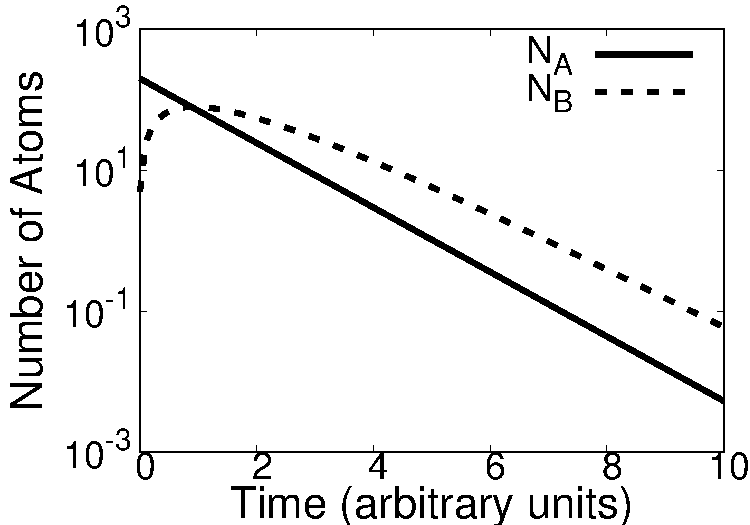
\includegraphics[width=\linewidth]{t_eq_1.pdf}
     \caption{$\tau_A / \tau_B=1$}
     \label{fig:tau_eq_1}
   \end{subfigure}
 ~
   \begin{subfigure}{.7\linewidth}
     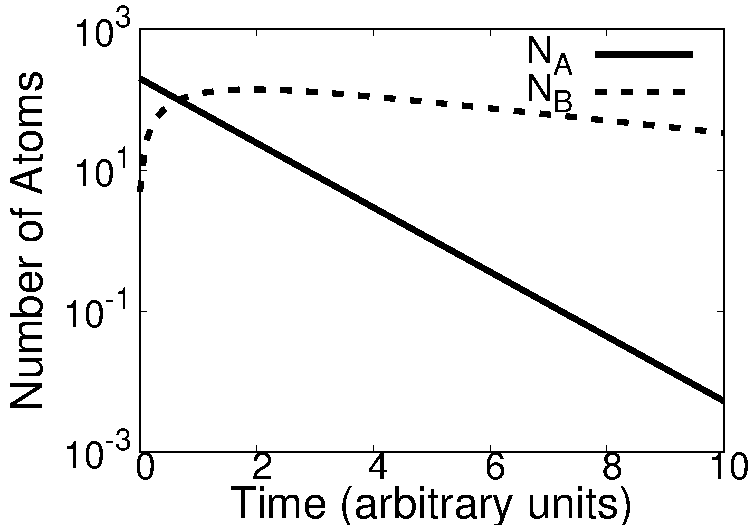
\includegraphics[width=\linewidth]{t_lt_1.pdf}
     \caption{$\tau_A / \tau_B=0.2$}
     \label{fig:tau_lt_1}
   \end{subfigure}

   \caption{Numerical solutions of $A$ and $B$ nucleus populations for various values of \trel.
   All figures generated with $dt=0.1$. Semilog axes are used to highlight the
   exponential decay of the populations.}
   \label{fig:numerical}
 \end{figure}

This is demonstrated in Figs.~\ref{fig:tau_gt_1}-\ref{fig:tau_lt_1}, which show
the $A$ population decaying at a constant rate regardless of the value of \trel.
These plots also show that decreasing \trel~decreases the slope of $N_B$,
in other words slowing the decay rate of the $B$ population.

Physically, this means that if the $B$ population has a longer e-folding time,
meaning it is more stable than the $A$ population, then the $B$ population decays
more slowly than the $A$ population.

Although varying \trel~changes the rate of decay of the $B$ population, each
regime exhibits qualitatively similar behavior. The $A$ population continuously
experiences exponential decay, while the $B$ population initially spikes before
beginning to exponentially decay. The initial spike in the $B$ population is
physically described by the initial population of $A$ nuclei rapidly decaying
into $B$ nuclei. Since the rate of decay of $A$ nuclei is also the rate of creation
of $B$ nuclei, the decay of $A$ initially outweighs the decay of $B$, and the $B$
population experiences a net growth.
As the population of $A$ nuclei approaches 0, however, fewer $A$ nuclei
are available to decay into $B$ nuclei, and the rate of creation of new $B$
particles decreases. Eventually, it falls below the rate of decay of $B$, and
the $B$ population begins its decay.


\begin{figure}
  \begin{subfigure}{.7\linewidth}
    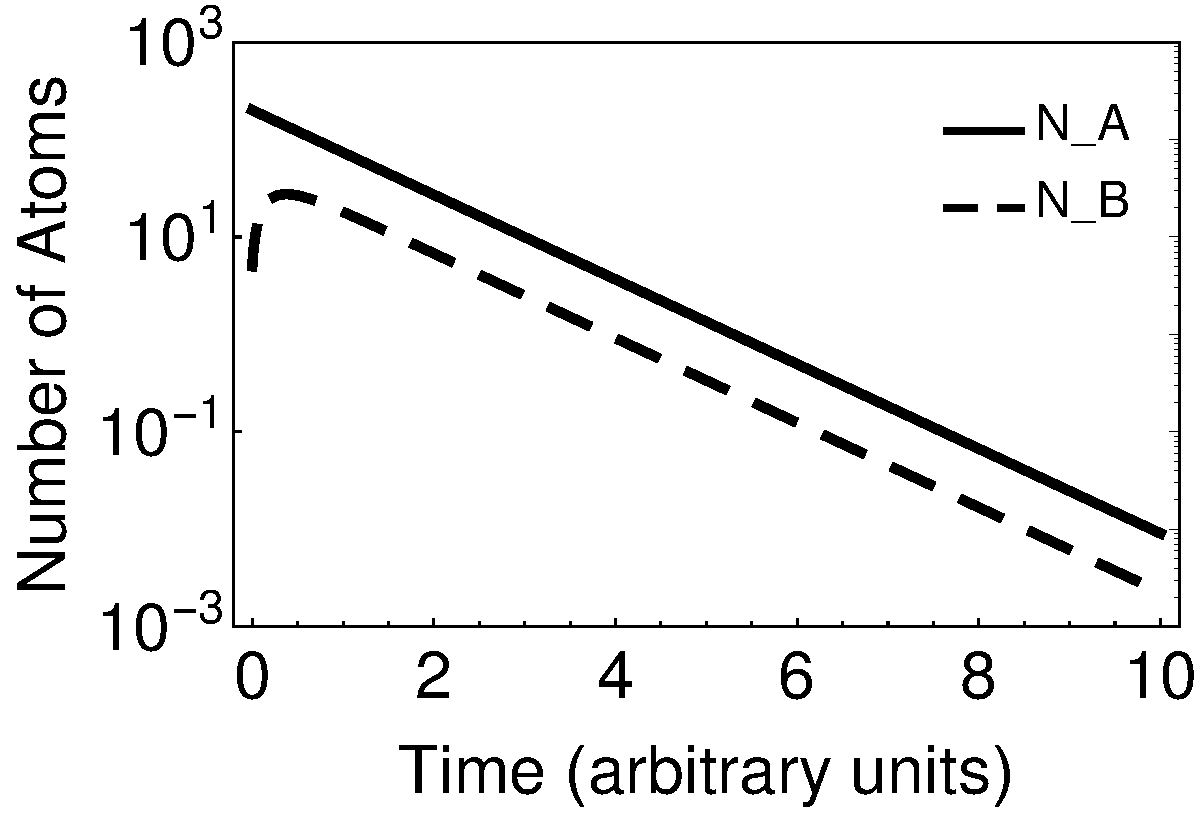
\includegraphics[width=\linewidth]{num_tgt1.pdf}
    \caption{$\tau_A / \tau_B=5$}
    \label{fig:tau_gt_1}
  \end{subfigure}
~
  \begin{subfigure}{.7\linewidth}
    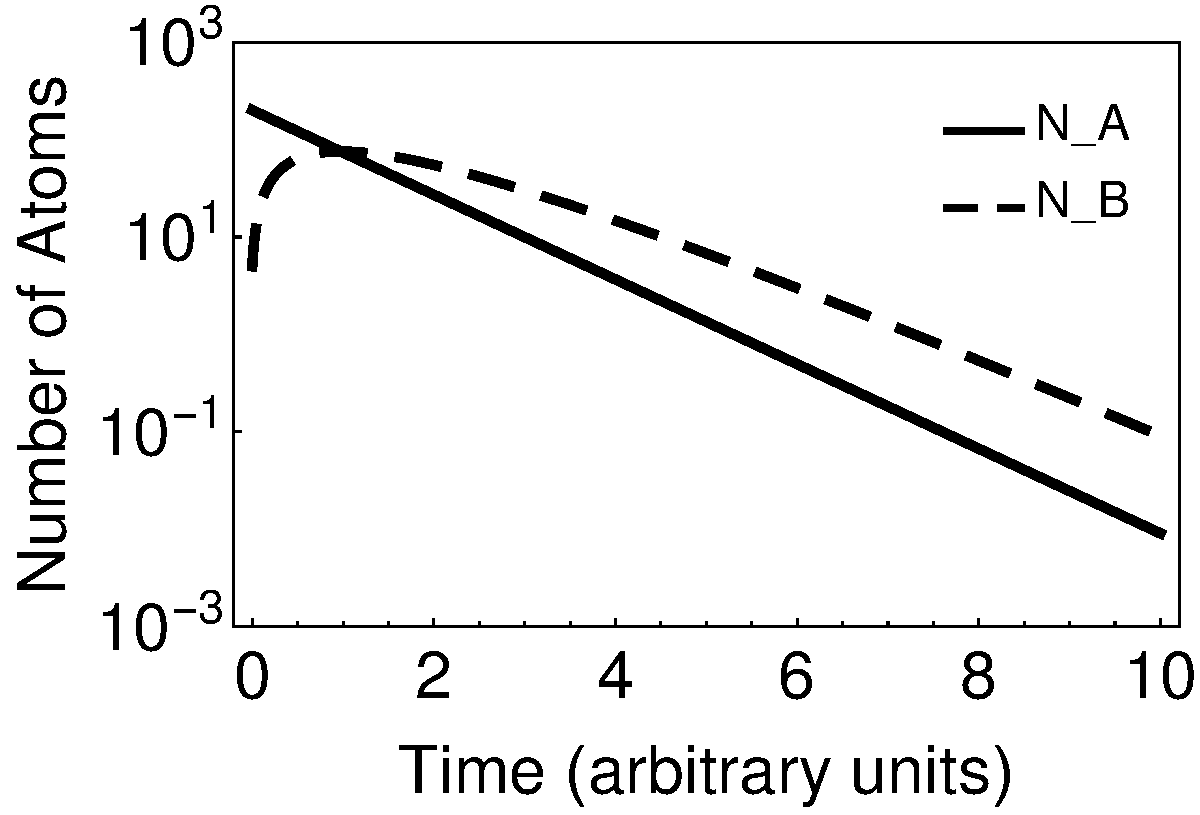
\includegraphics[width=\linewidth]{num_teq1.pdf}
    \caption{$\tau_A / \tau_B=1$}
    \label{fig:tau_eq_1}
  \end{subfigure}
~
  \begin{subfigure}{.7\linewidth}
    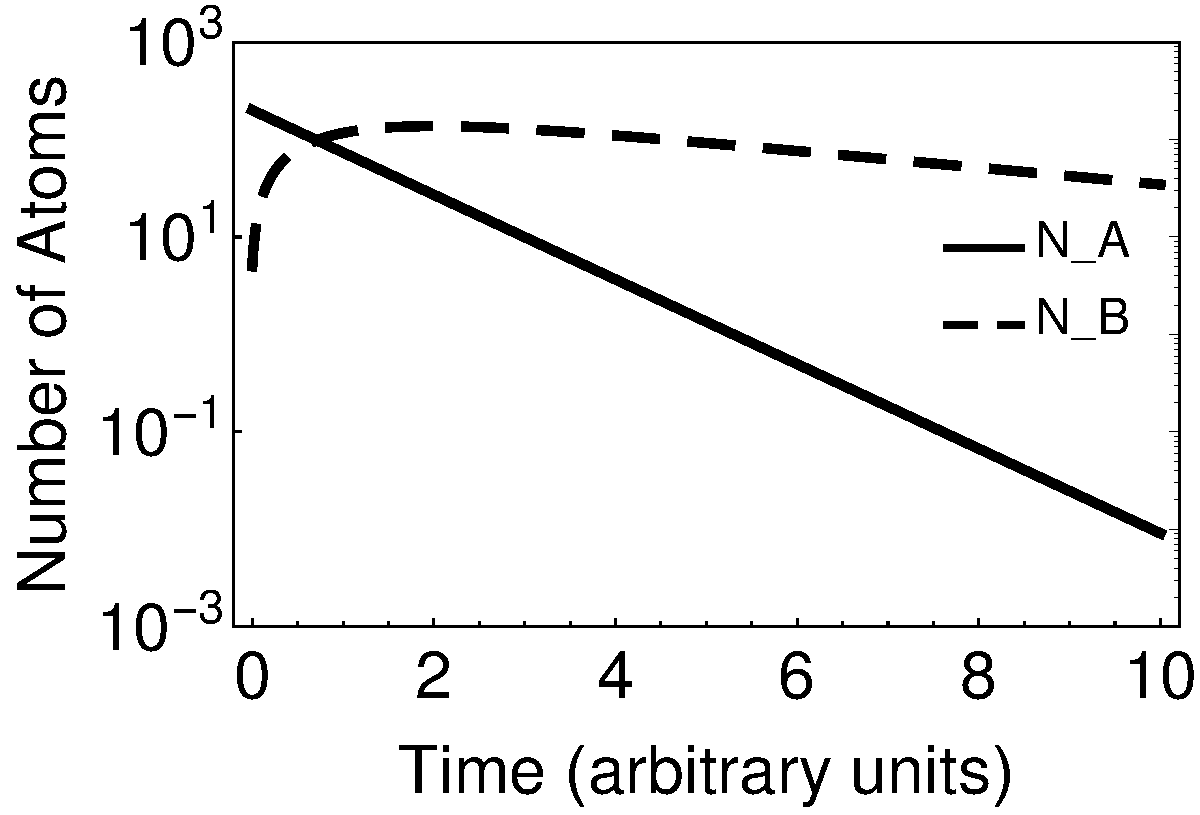
\includegraphics[width=\linewidth]{num_tlt1.pdf}
    \caption{$\tau_A / \tau_B=0.2$}
    \label{fig:tau_lt_1}
  \end{subfigure}

  \caption{Analytical solutions of $A$ and $B$ nucleus populations for various values of \trel.
  As in Fig.~\ref{fig:numerical}, semilog axes are used to highlight the
  exponential decay of the populations.}
  \label{fig:analytical}
\end{figure}

\subsubsection{Stability Analysis}\label{sec:stability}

It is also interesting to analyze the stability of this numerial analysis for
different timestep lengths $dt$. In Figs.~\ref{fig:tau_gt_1}-\ref{fig:tau_lt_1},
$dt=0.1$ is much smaller than the characteristic timescales of the system defined
by $\tau_A$ and $\tau_B$. As a result, we observe smooth curves, without obvious
inaccuracies caused by numerical instability.

Additionally, we can note that the most rapid change in the system occurs between
$t=0$ to $t=1$, after which $N_B$ settles into a constant
rate of exponential decay. So, while $dt$ is short enough to capture the dynamics
of this time, i.e. smaller than order $1$, we expect stable results.

\begin{figure}
  \begin{subfigure}{.8\linewidth}
    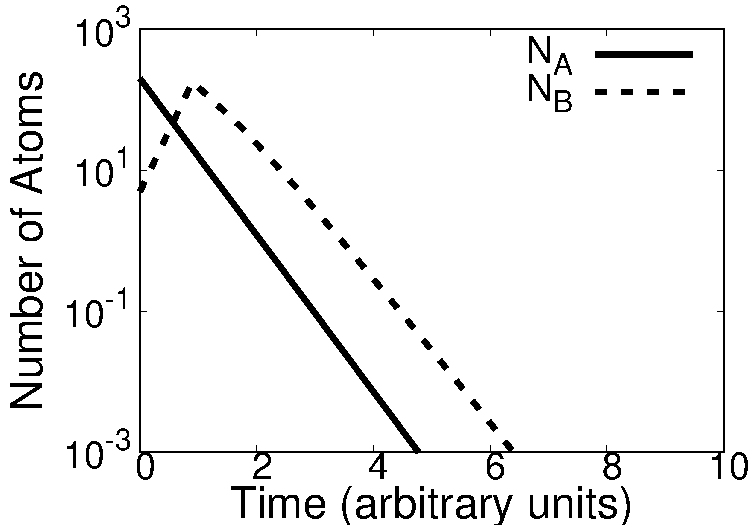
\includegraphics[width=\linewidth]{t_eq_1_unstable.pdf}
    % \caption{ With $dt=0.9$,
    % instability in analysis causes the system to decay abnormally quickly.}
    \caption{ $dt = 0.9$ }
    \label{fig:tau_eq_1_unstable}
  \end{subfigure}

  \begin{subfigure}{.8\linewidth}
    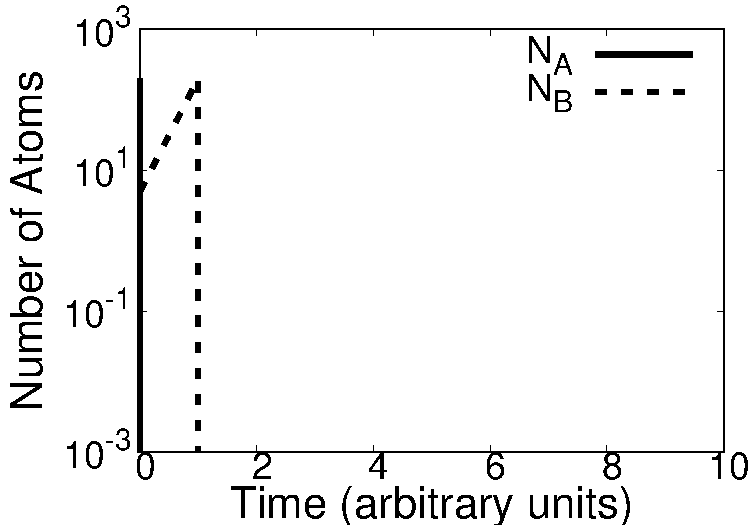
\includegraphics[width=\linewidth]{t_eq_1_vunstable.pdf}
    % \caption{With $dt=1.0$, instability is even more prominent, and populations immediately go
    % to 0.}
    \caption{$dt=1.0$}
    \label{fig:tau_eq_1_vunstable}
  \end{subfigure}

  \caption{Plots of \trel~$ = 1$ as in Fig.~\ref{fig:tau_eq_1} with $dt$ varied
  to demonstrate instability in numerical analysis. Setting $dt$ to the
  order of \trel~introduces an instability that causes
  the populations to drop to 0 abnormally quickly.}
\end{figure}

We can verify this by varying the timestep length about \trel. In Fig.~\ref{fig:tau_eq_1_unstable}
$dt$ is set to $0.9$, just slightly below the timescale on which the initial increase
in the $B$ population occurs. Compared to Fig.~\ref{fig:tau_eq_1}, the decay
is much quicker, and the initial growth of $B$ is linear rather than damped
decreasing exponential growth.

Fig.~\ref{fig:tau_eq_1_vunstable} shows an even more exaggerated example of this,
where $dt = \tau_A / \tau_B$. In this case, when the second step of the simulation
is calculated, the long time step and negative first derivatives from the initial
conditions bring both populations to 0.

Another type of instability exists only the $\tau_A / \tau_B > 1$ case.
Shown in Fig.~\ref{fig:tgt1_unstable}, this oscillatory instability only appears
in this particular regime of \trel. This is particularly unphysical, since it
describes a negative population of $B$ nuclei. Here, this instability is present
in approximately the range $.35 < dt < .5$, below which the model is stable,
and above which it exhibits the same sharp instability present in Fig.~\ref{fig:tau_eq_1_vunstable}.

\begin{figure}
  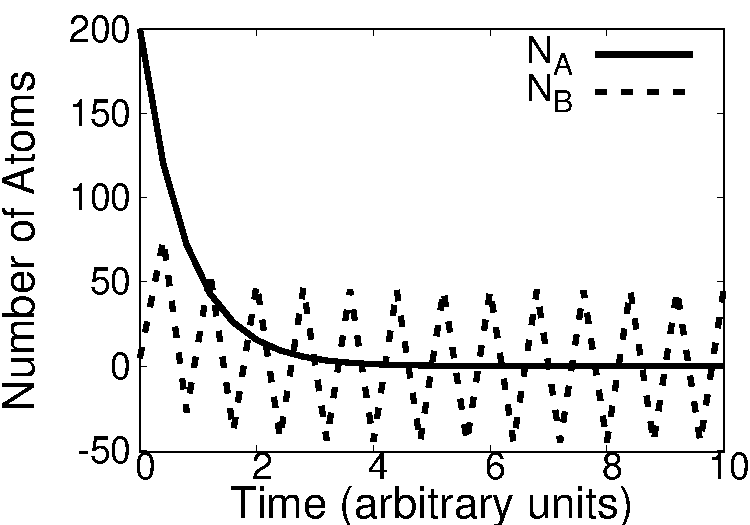
\includegraphics[width=.8\linewidth]{tgt1_osc.pdf}
  \caption{Oscillatory instability in the numerical solution when \trel$=5$
  and $dt=0.4$.}
  \label{fig:tgt1_unstable}
\end{figure}



\subsection{Part II - Resonance}\label{sec:resonance}

Examining the resonant system shows a different behavior, where a nonzero
steady state is reached for the populations. Eqs.~\ref{eq:res_A_norm} and
\ref{eq:res_B_norm} show that the $N_B$ population has twice the e-folding time of
the $N_A$ population, evidenced by the $2 \tau$ in the denominator of the $N_B$
terms. We can see that the time derivatives of each population is equal to 0
when $N_B = 2 N_A$, indicating the populations have reached their equilibrium
states.

We see this manifested in Figs.~\ref{fig:resonance} and \ref{fig:analyt_resonance},
where the $N_B$ population is stably twice that of the $N_A$ population at long times.
Particles tunnel out of the $A$ state more rapidly than the $B$ state, leaving
fewer particles in the $A$ state at any time.

\begin{figure}

  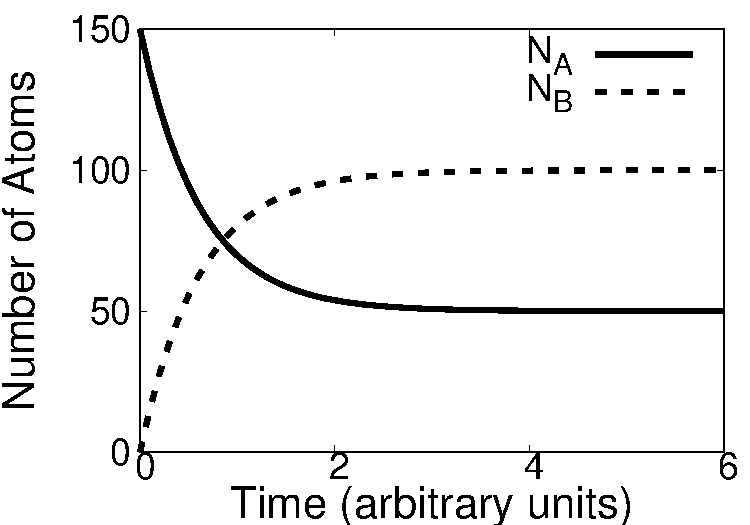
\includegraphics[width=.8\linewidth]{resonance.pdf}
  \caption{Numerical solution to the resonance problem. The system exhibits steady
  state behavior when $N_B = 2 N_A$.}
  \label{fig:resonance}
\end{figure}
\begin{figure}

  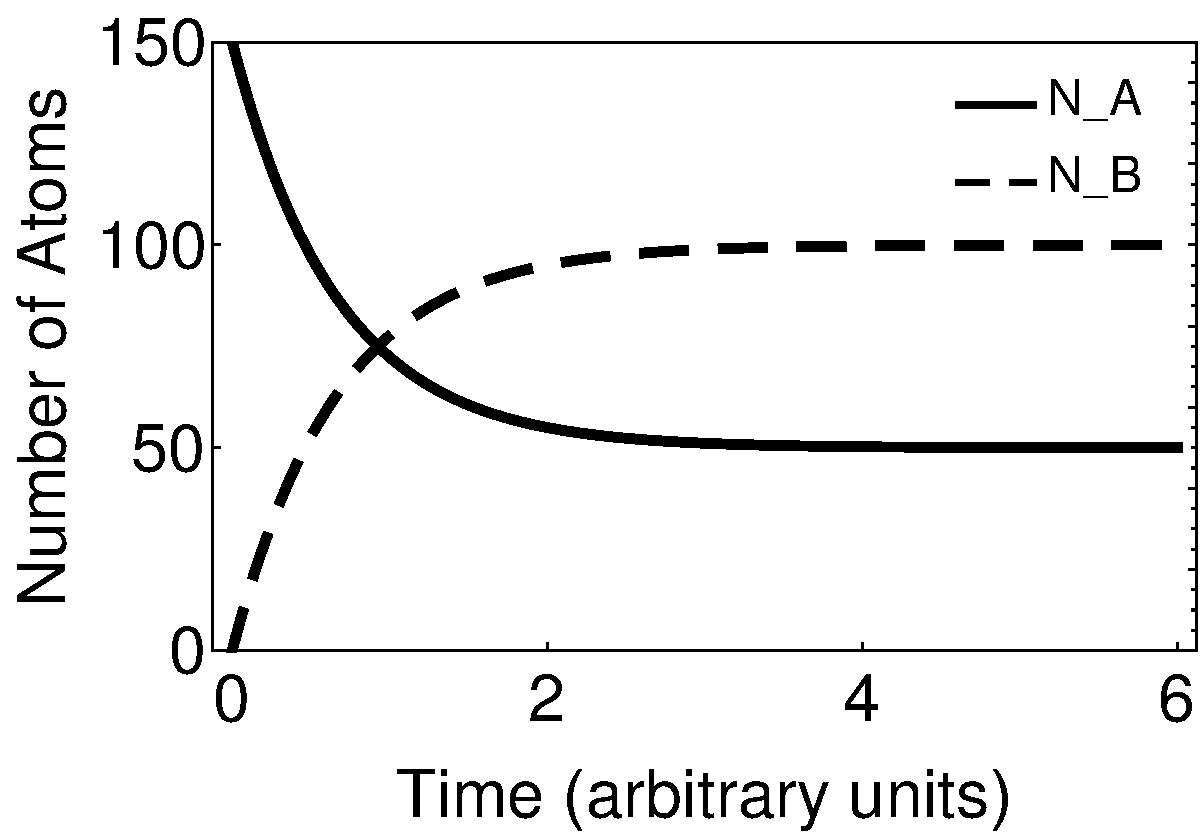
\includegraphics[width=.8\linewidth]{analyt_res.pdf}
  \caption{Exact solution to the resonance problem. The same steady
  state behavior where $N_B = 2 N_A$ as in Fig.~\ref{fig:resonance} is visible.}
  \label{fig:analyt_resonance}
\end{figure}


\section{Conclusions} \label{sec:conclusion}

In Section~\ref{sec:decay}, numerical solutions to a radioactive decay problem
are examined in three different regimes of \trel. The normalized equations
Eqs.~\ref{eq:decay_A_norm} and \ref{eq:decay_B_norm} indicate that the $A$ population
has no dependence on \trel, and that the $B$ population's rate of decay will
decrease as \trel~decreases. This is examined and confirmed in the cases where \trel$<1$,
\trel$=1$, and \trel$>1$.

The stability of the numerical solutions to the radioactive decay problem is
investigated in Section~\ref{sec:stability}. For \trel$<=0$, the solution is
stable when $dt$ is smaller than the order of \trel. For \trel$>0$, an
oscillatory instability is also present for a certain range of $dt$. Below this
range, the solution is stable, and above this, the same instability as before exists.

Finally, a resonant system where particles tunnel between two energy states
is modelled in Section~\ref{sec:resonance}. It is found that the system reaches
a steady state where $N_B = 2 N_A$. Examining Eqs.~\ref{eq:res_A_norm} and
\ref{eq:res_B_norm} which describe this system, we confirm that the time
derivatives of each population go to 0 when $N_B = 2 N_A$.

\begin{thebibliography}{1}

\end{thebibliography}

\end{document}
